\documentclass[a4paper, 12pt]{article}

\usepackage{wrapfig}
\usepackage{graphicx}
\usepackage{mathtext}
\usepackage{amsmath}
\usepackage{siunitx}
\usepackage{multirow}
\usepackage{rotating}

\usepackage[T1,T2A]{fontenc}

\usepackage[russian]{babel}

\graphicspath{{pictures/}}


\usepackage[left=0.9cm,right=0.7cm,
    top=0.7cm,bottom=0.7cm,bindingoffset=0cm]{geometry}
\begin{document}
\begin{center}
    

\begin{figure}[h!]
        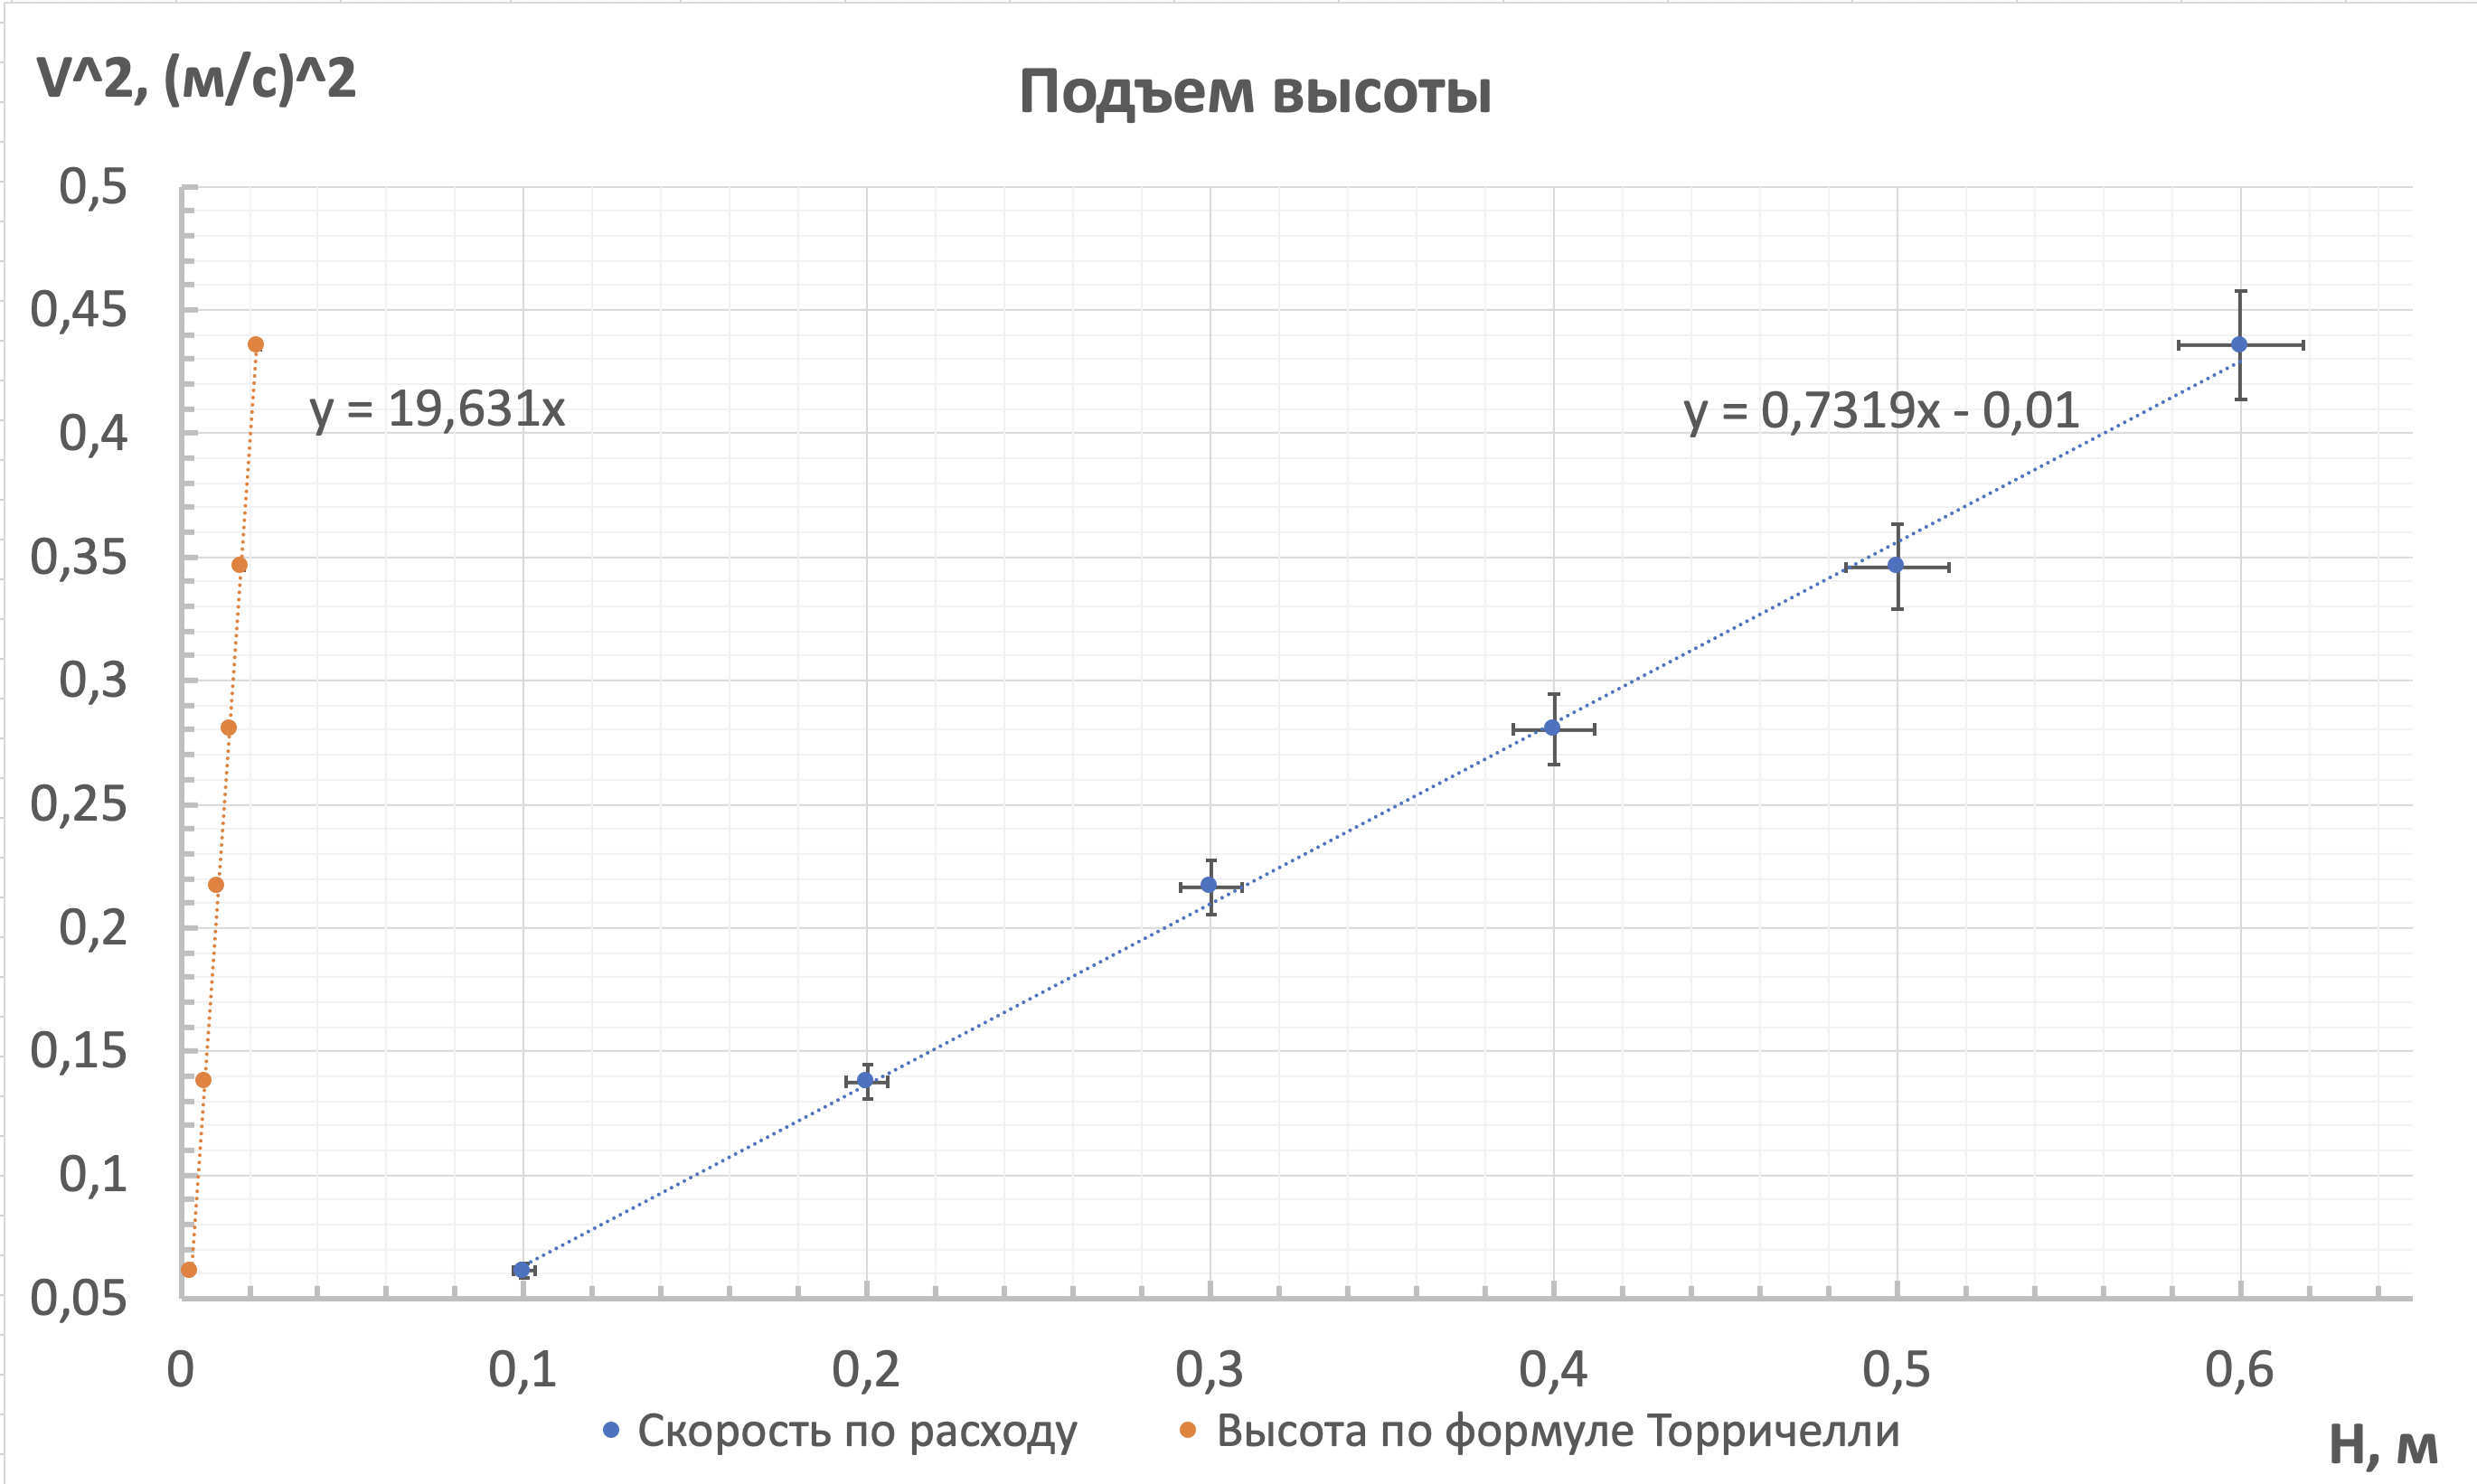
\includegraphics[width=1.0\textwidth]{graph1.png}
        \caption{Скорости по расходу (подъем)}
        \label{ris:ustanovka}
    \end{figure}

\begin{figure}[h!]
        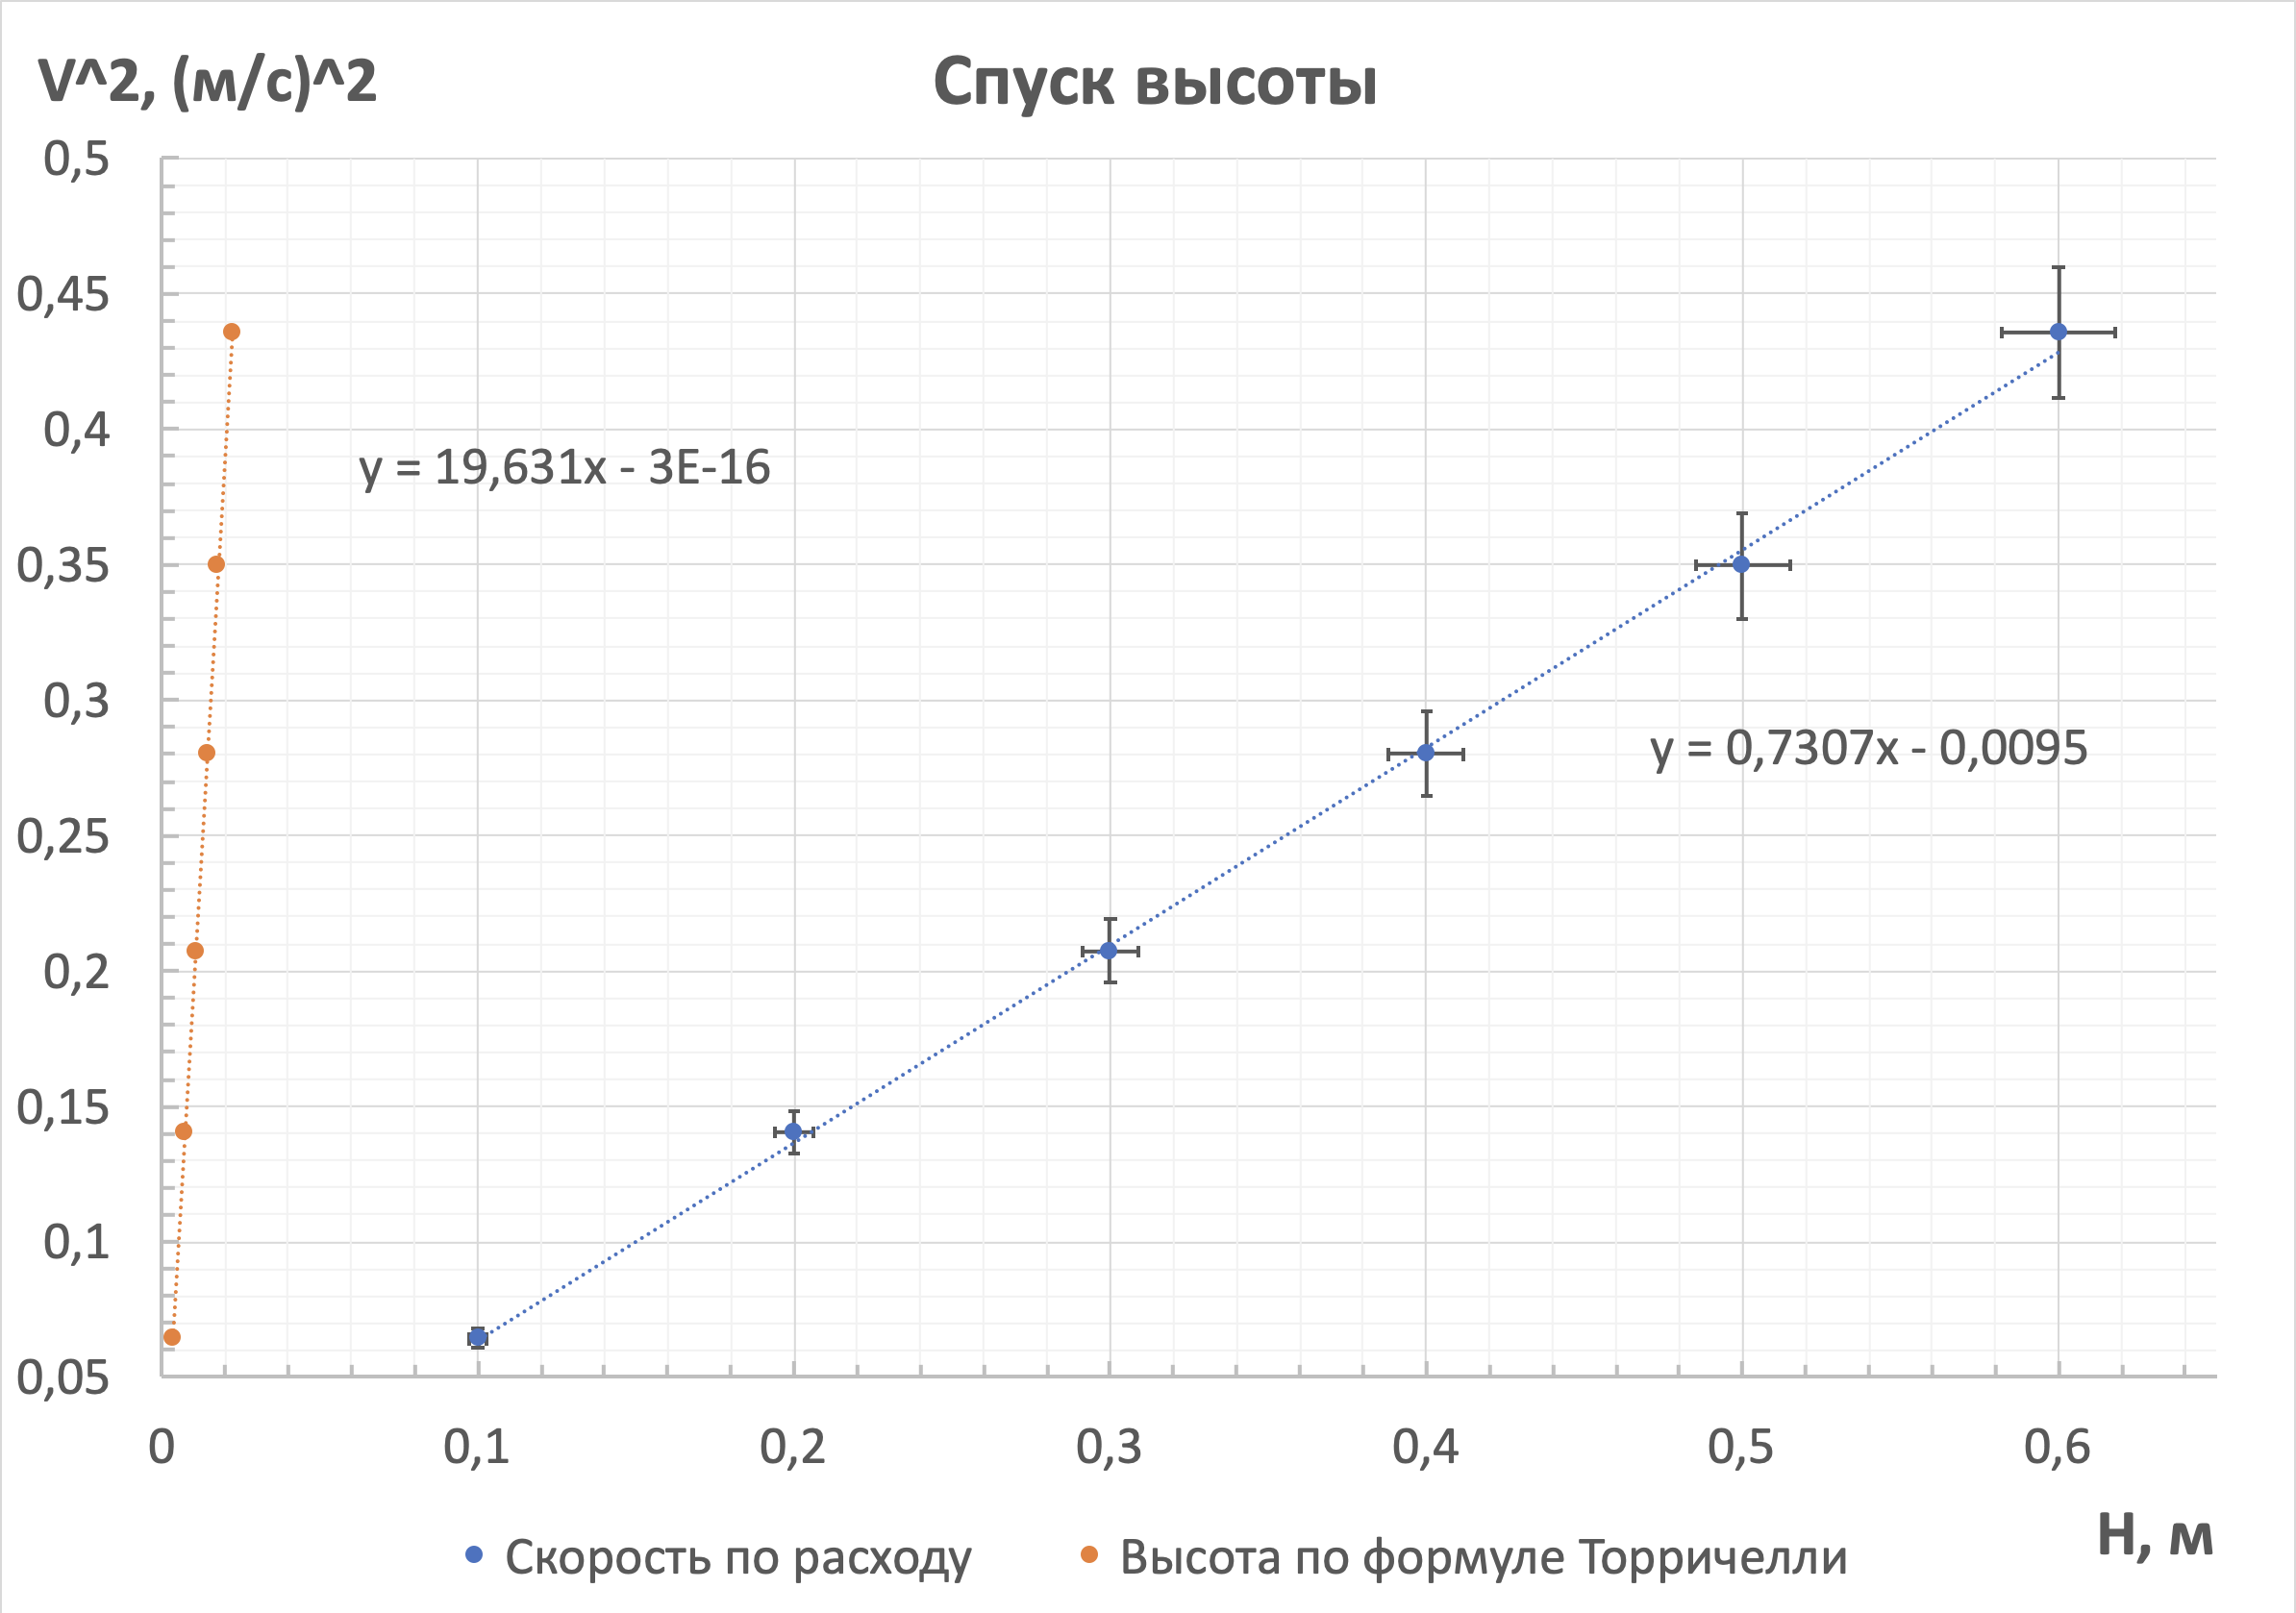
\includegraphics[width=0.94\textwidth]{graph2.png}
        \caption{Скорости по расходу (спуск)}
        \label{ris:ustanovka}
    \end{figure}

\begin{figure}[h!]
        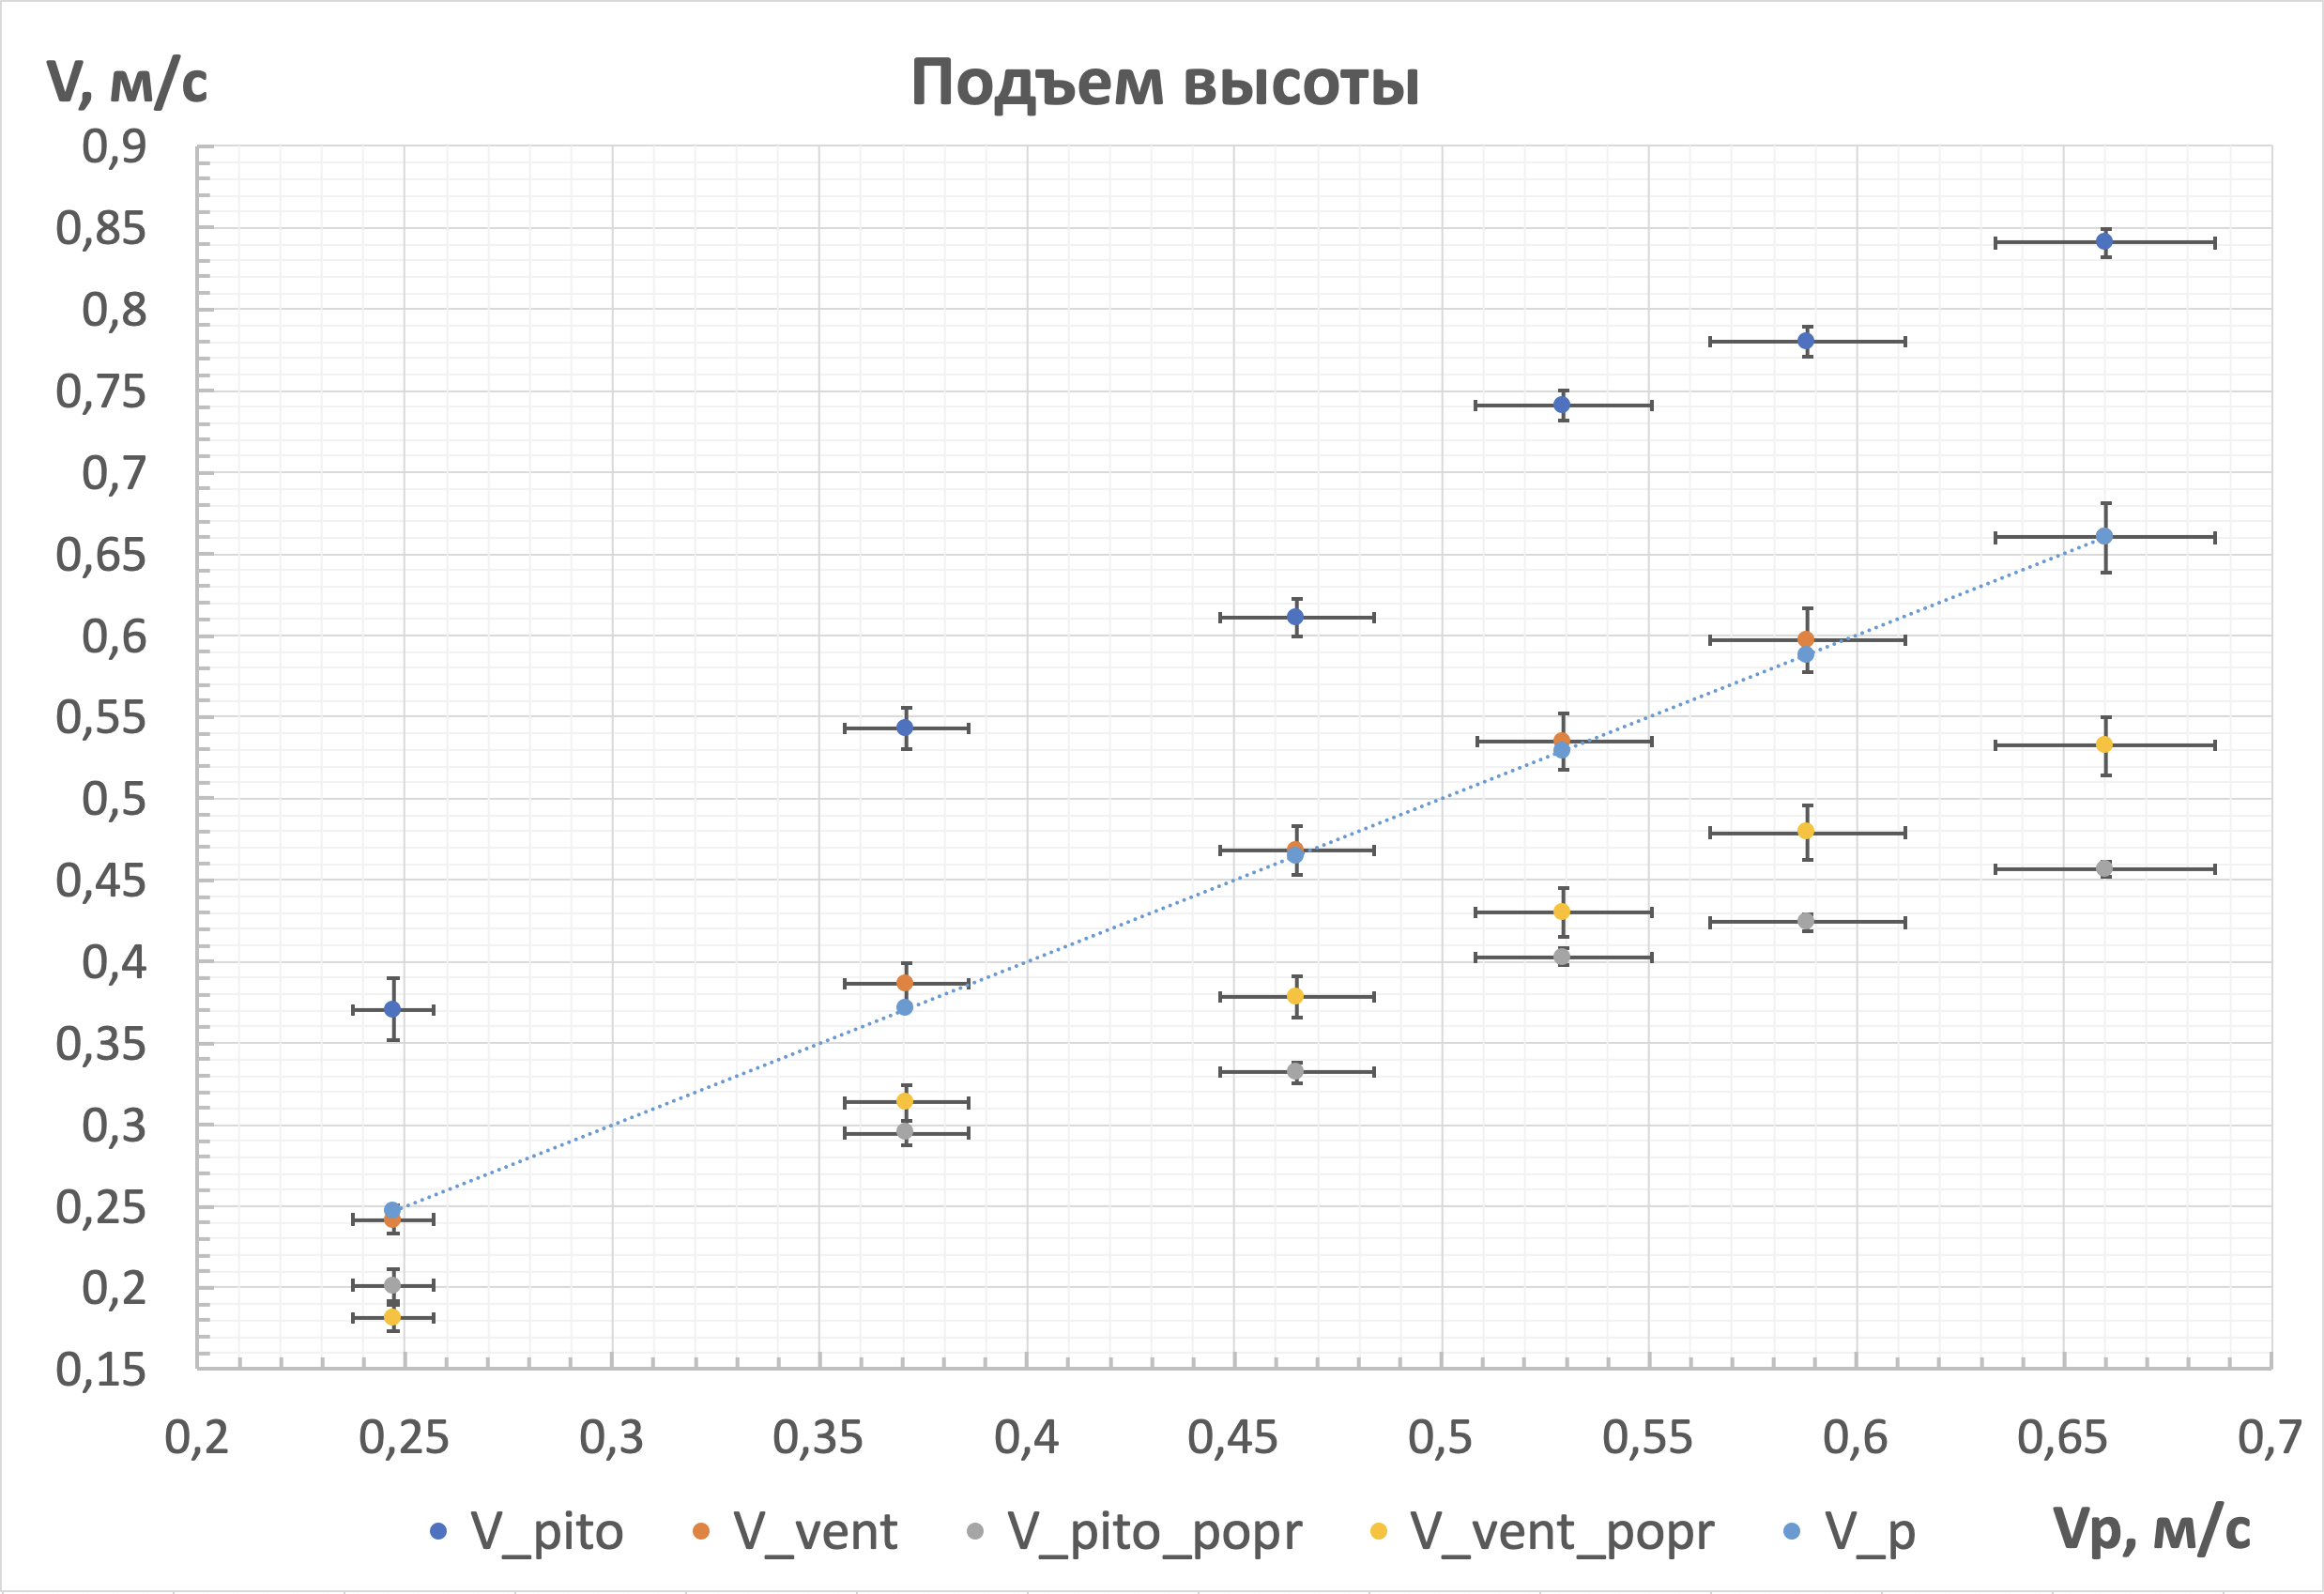
\includegraphics[width=0.92\textwidth]{graph3.png}
        \caption{Скорости по расходомерам Пито и Вентури (подъем)}
        \label{ris:ustanovka}
    \end{figure}


\begin{figure}[h!]
        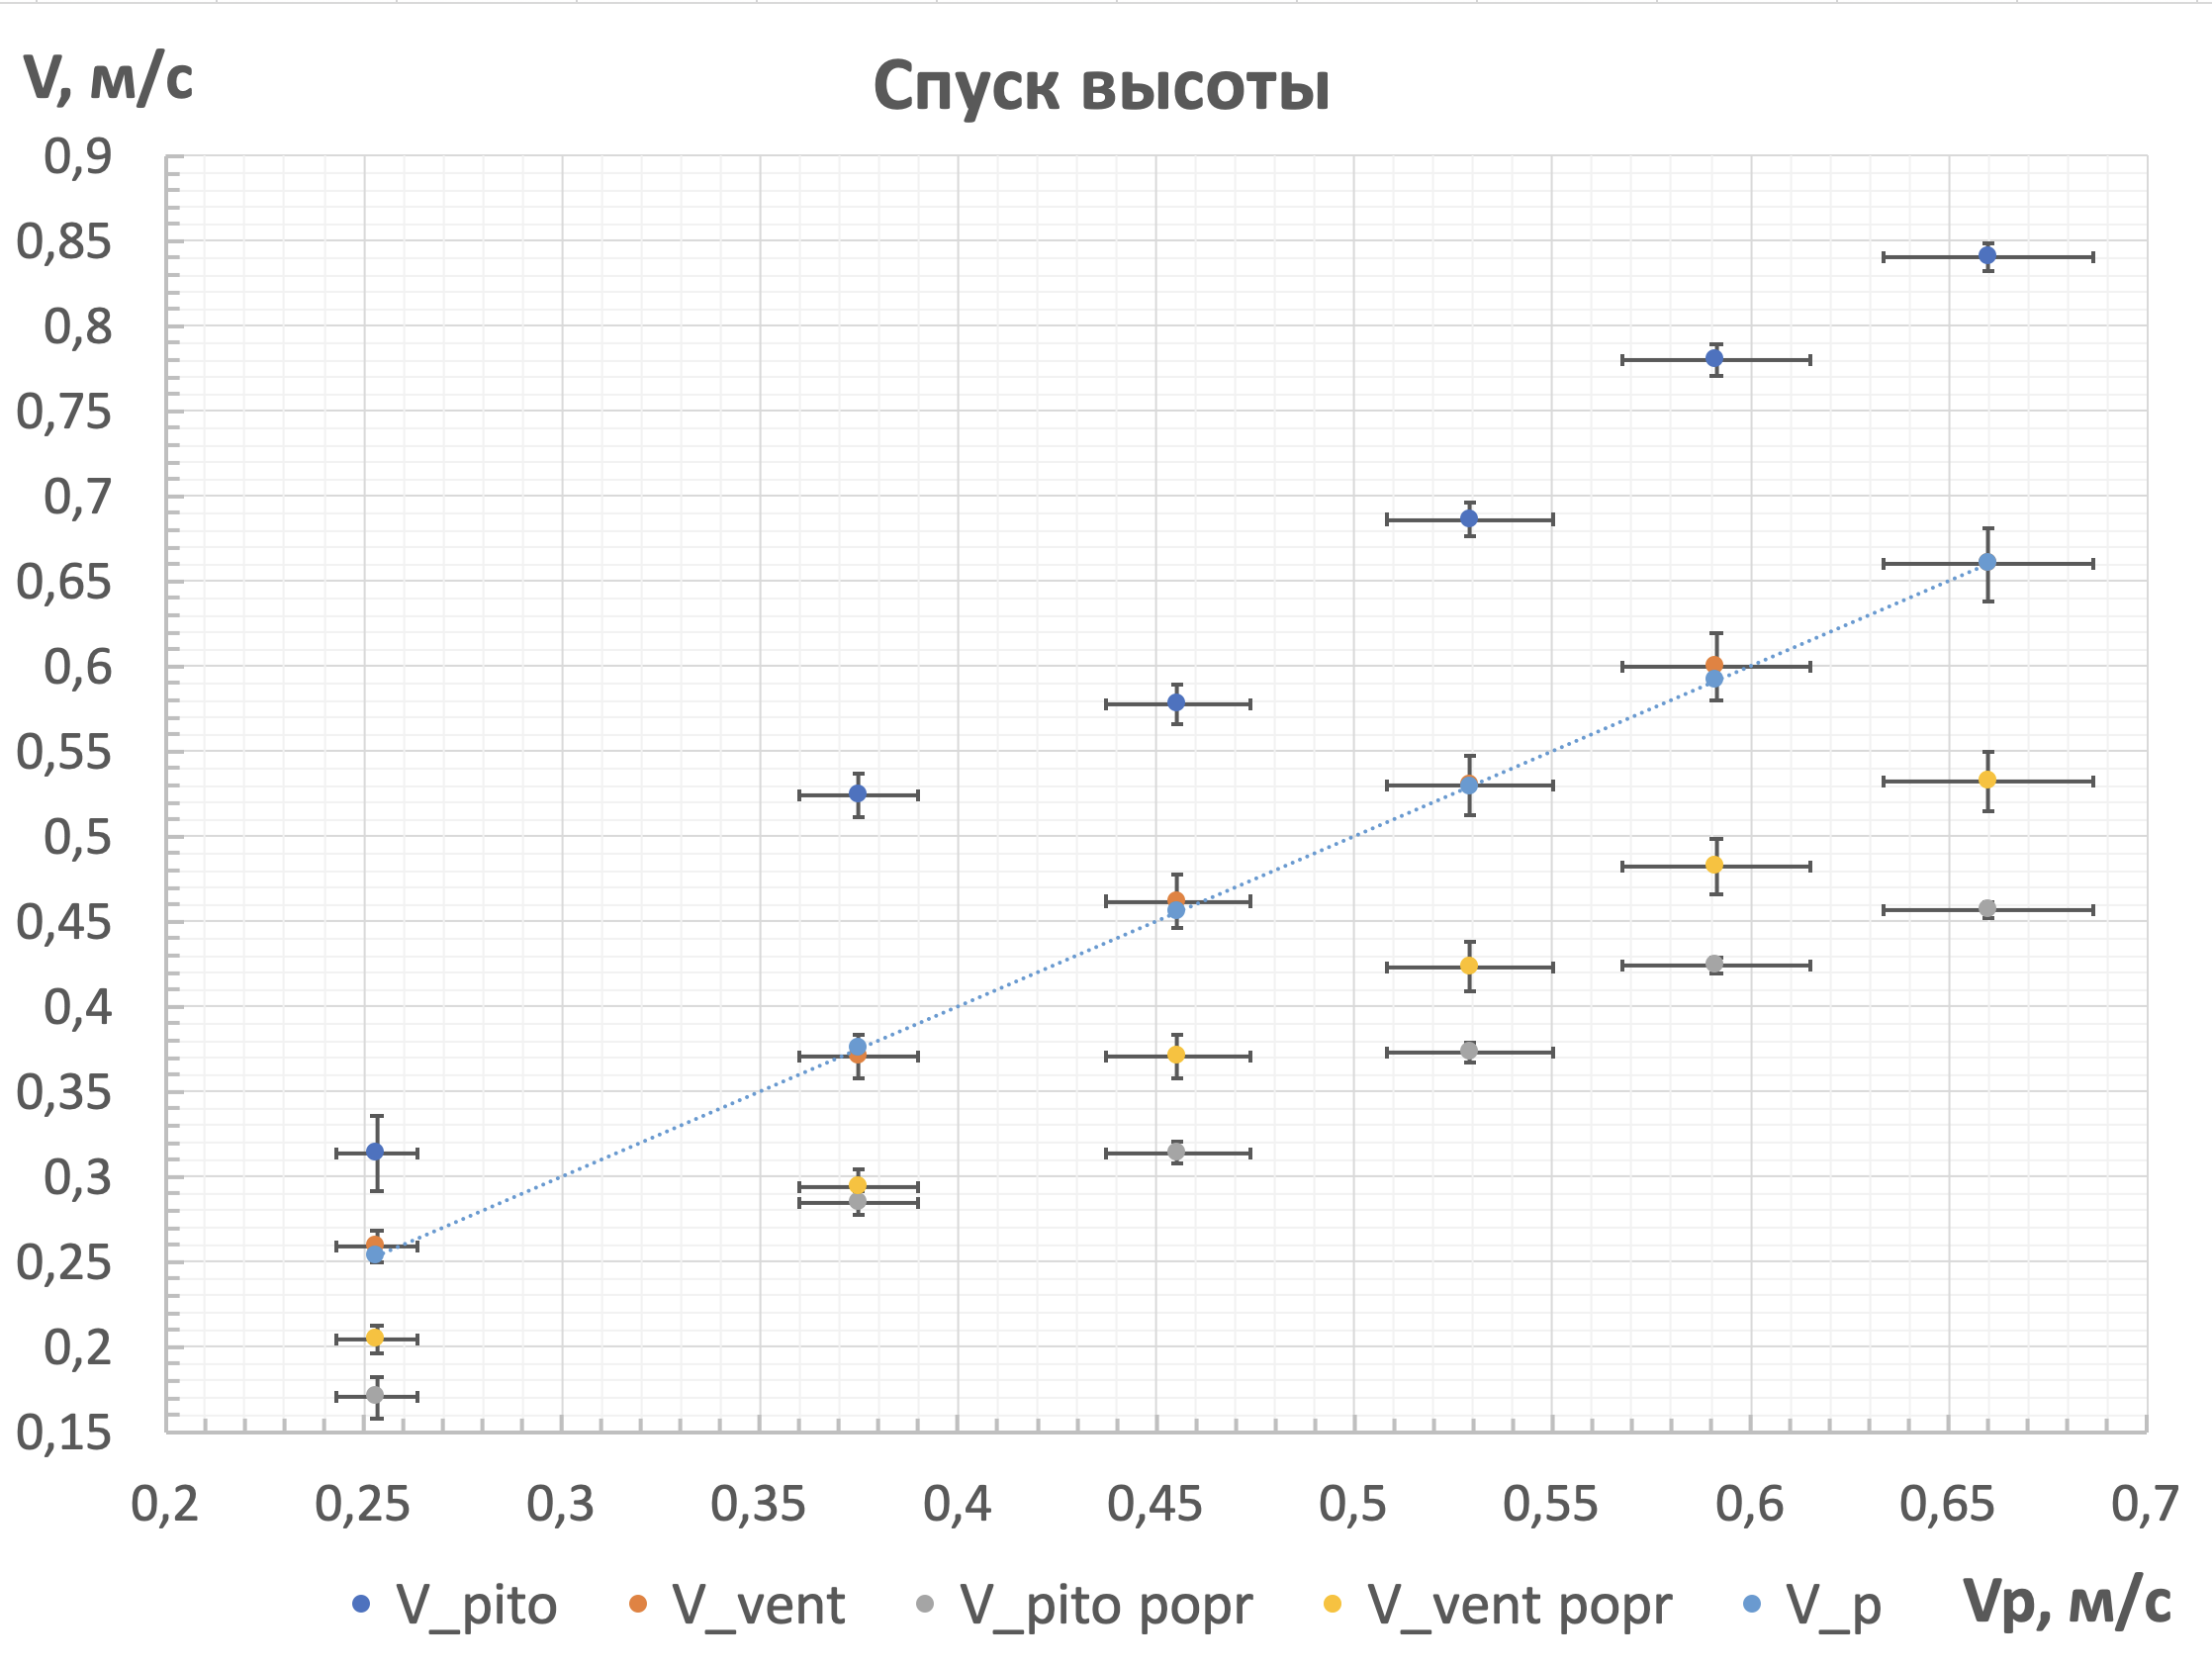
\includegraphics[width=0.92\textwidth]{graph4.png}
        \caption{Скорости по расходомерам Пито и Вентури (спуск)}
        \label{ris:ustanovka}
    \end{figure}
    
\begin{figure}[h!]
        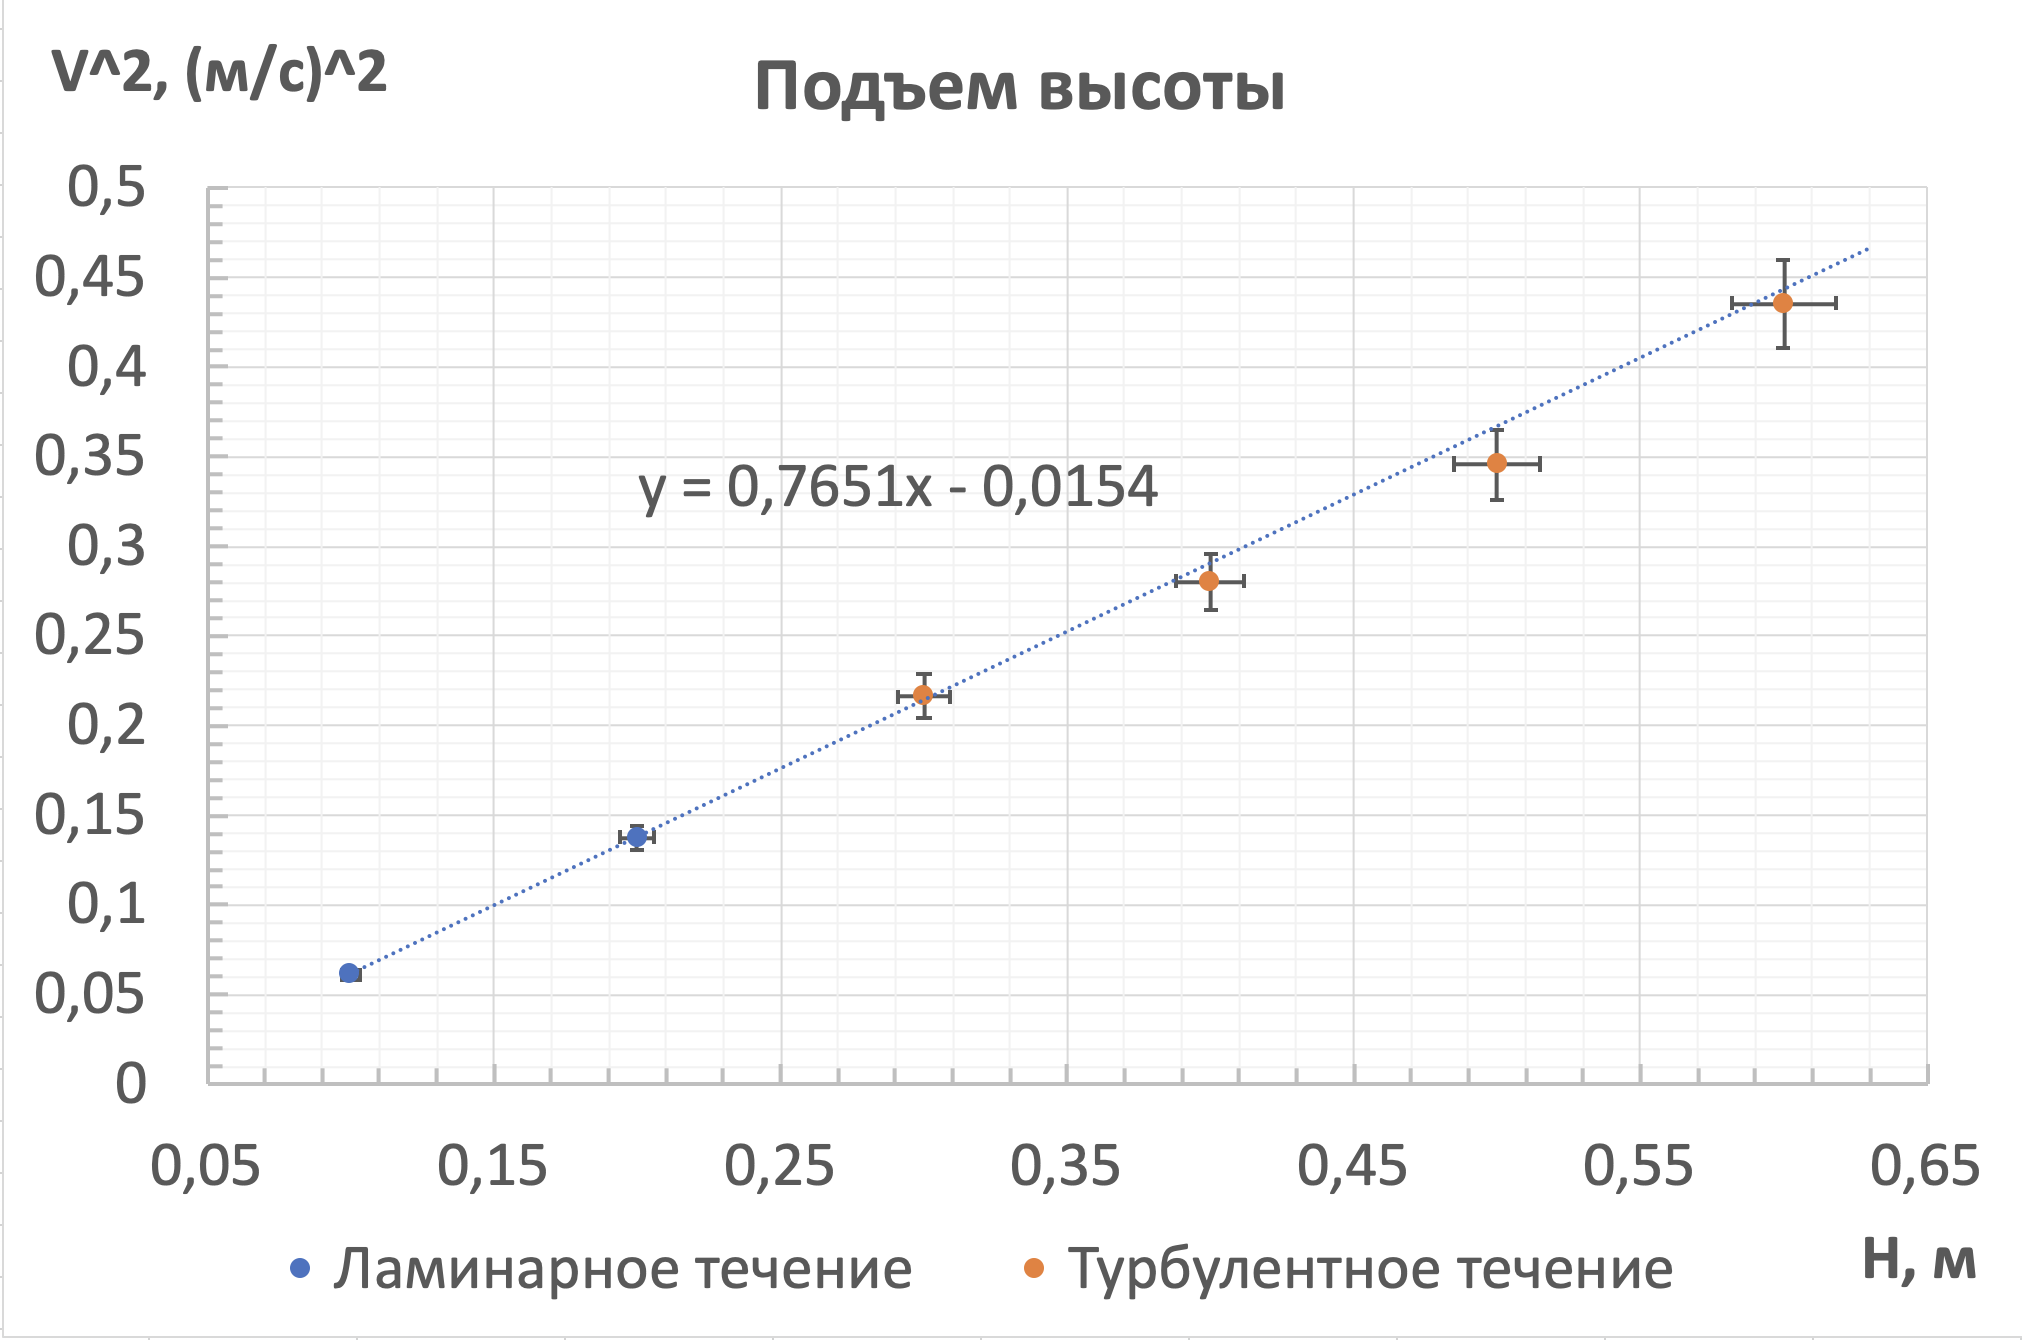
\includegraphics[width=0.91\textwidth]{graph5.png}
        \caption{Определение чисел Рейнольдса (подъем)}
        \label{ris:ustanovka}
    \end{figure}


\begin{figure}[h!]
        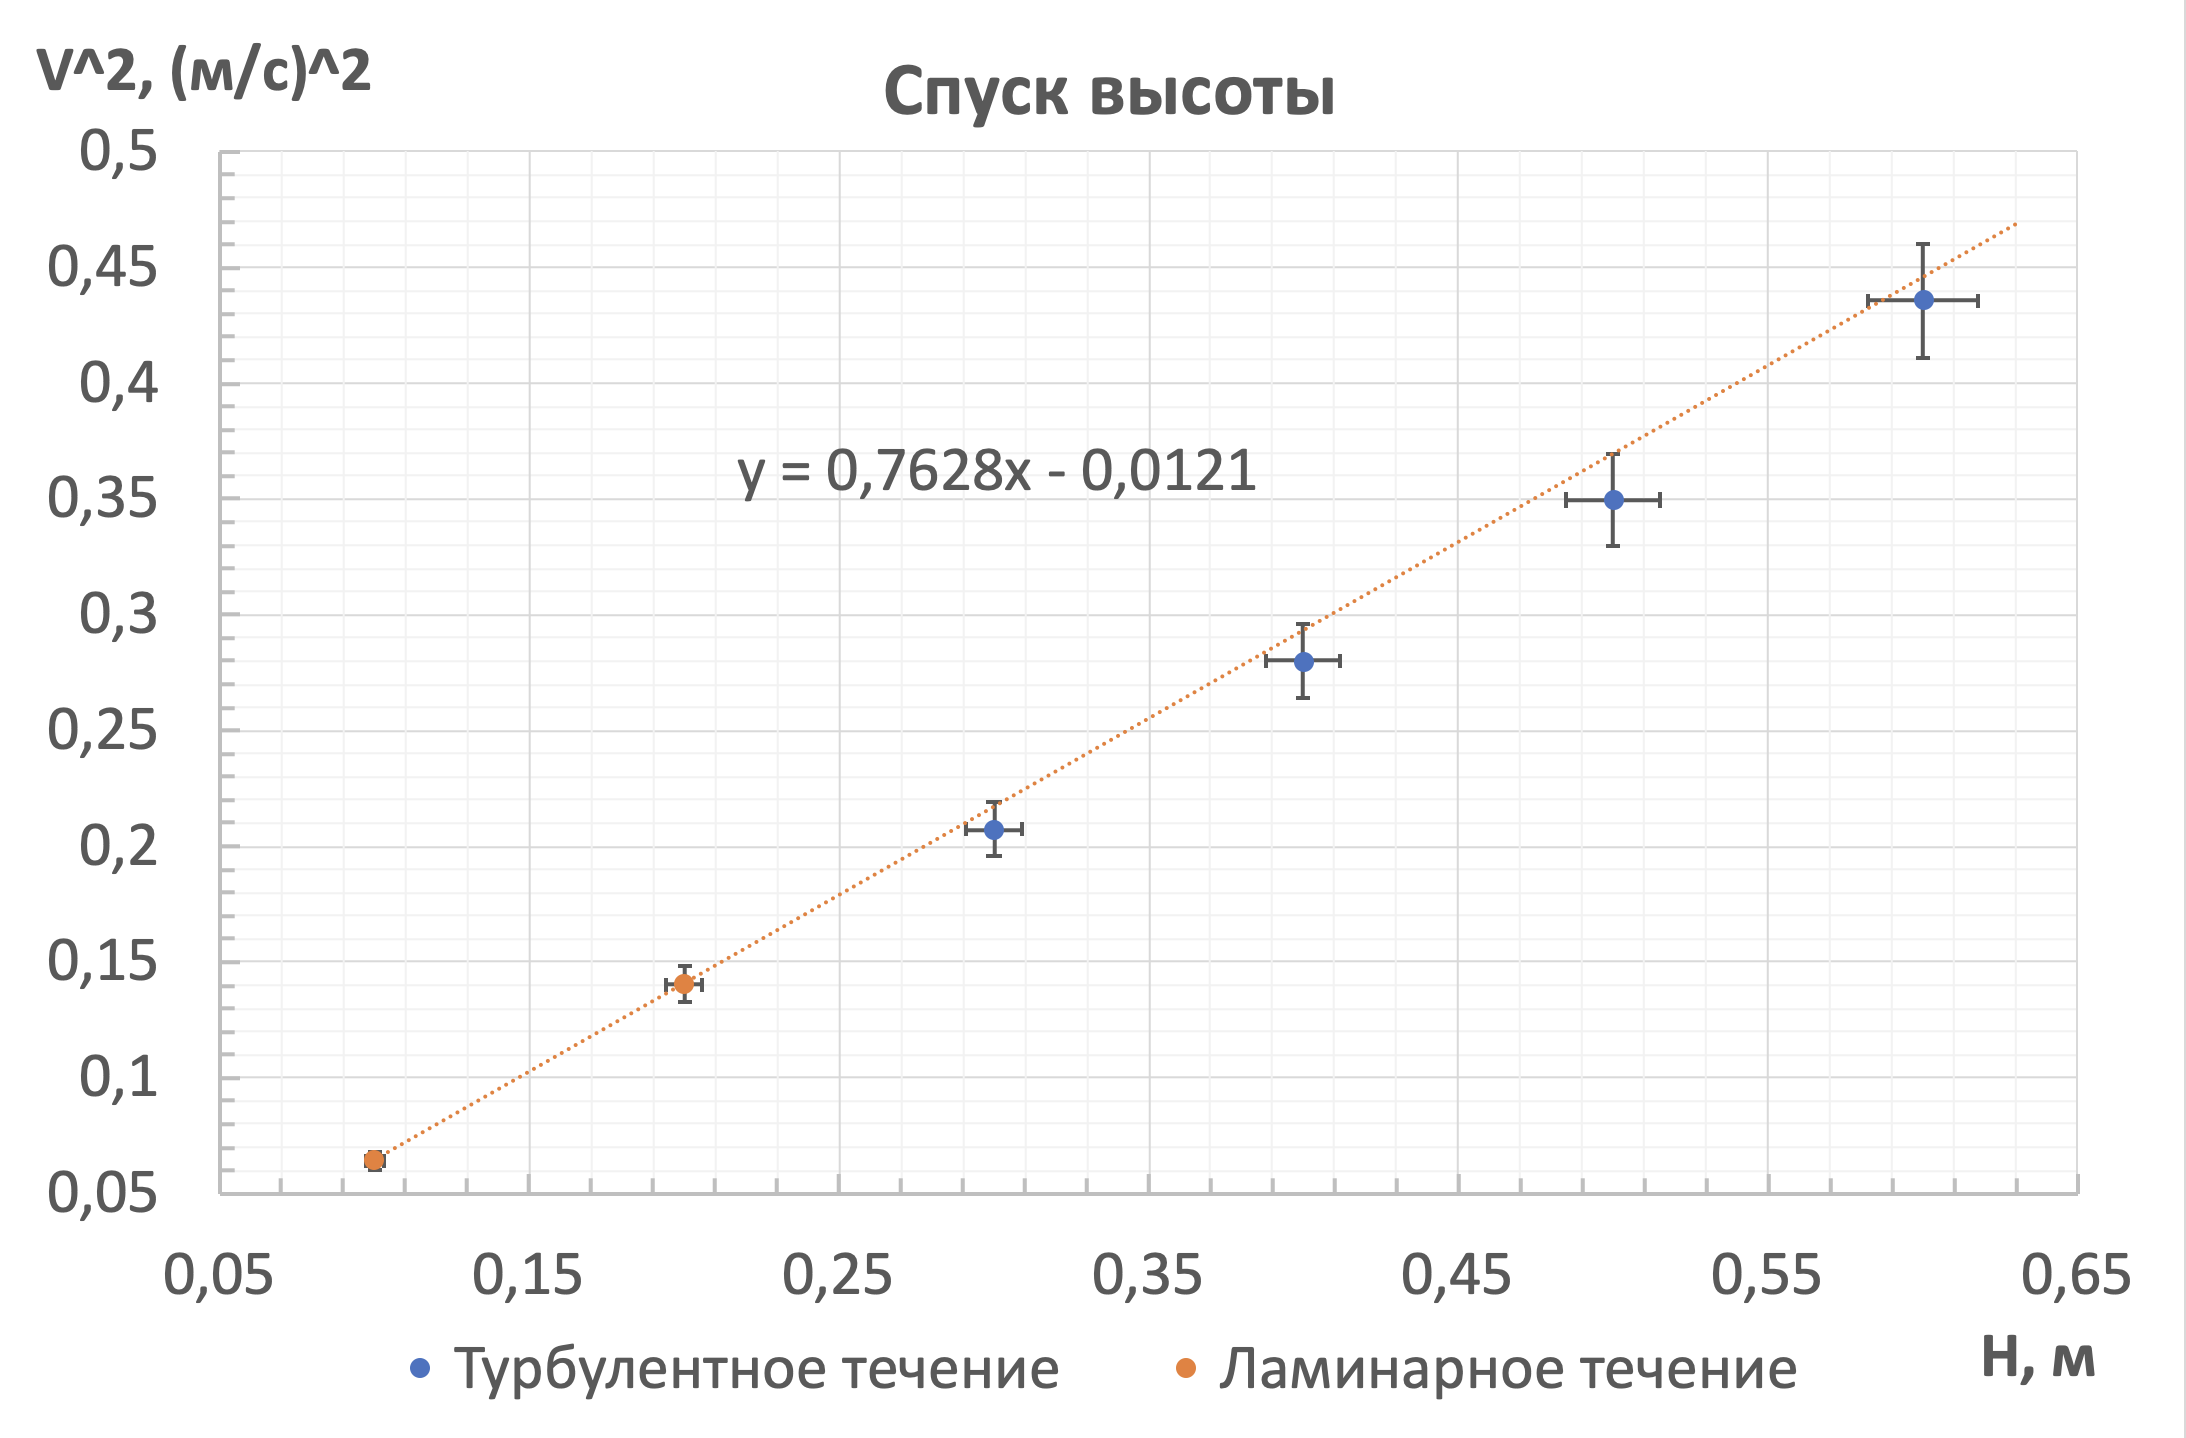
\includegraphics[width=0.91\textwidth]{graph6.png}
        \caption{Определение чисел Рейнольдса (спуск)}
        \label{ris:ustanovka}
    \end{figure}
\end{center}
\end{document}
